\documentclass{crypto-exercise}
\usepackage{amsthm}
\usepackage{pgfplots}
\usepackage{tikz}
\author{Sven Laur}
\contributor{Sven Laur}
\tags{semantic-security, coin-fixing argument}


\begin{document}
\begin{exercise}{Coin-fixing and semantic-security}
Let $\SSS$ be a distribution of secret values. Then the semantic security of a function $f$ against predicting a function $g$ is defined through an advantage
\begin{align*}
   \advSemXX{f,g}{\AD}%
   &=\pr{s\gets\SSS:\AD(f(s))=g(s)}
   -\max_{y_*\in\YYY}\pr{s\gets\SSS:g(s)=y_*}\enspace.
\end{align*}
Show that we cannot a priory postulate that deterministic functions are easier to predict. In particular, show that there may exist $\AD$ and a randomised function $g:\SSS\times\Omega\to\YYY$ such that   
\begin{align}
\label{eq:bound}
\advSemXX{f,g}{\AD}\leq \max_{\omega\in\Omega} \set{\advSemXX{f,g_\omega}{\AD}}
\end{align}
where $g_\omega:\SSS\to\YYY$ is a deterministic function defined as $g_\omega(s)=g(s,\omega)$. \end{exercise}

\begin{solution}
Let us first express definitions in terms of corresponding security games. The advantage $\advSemXX{f,g}{\AD}$ can be expressed as the distance between the following games
\begin{align*}
&\begin{game}{\GAME_0}
&s\gets\SSS\\
&x\gets f(s)\\
&\RETURN [\smash{g(s)\iseq\AD(x)}] 
\end{game}
&&\begin{game}{\GAME_1}
&s\gets\SSS\\
&x\gets f(s)\\
&\RETURN [\smash{g(s)\iseq y_*}] 
\end{game}
\end{align*}
where $y_*$ is the must probable outcome of $g(s)$. Now for a fixed random value $\omega$, the advantage 
$\advSemXX{f,g_\omega}{\AD}$ can be expressed as the distance between the following games
\begin{align*}
&\begin{game}{\GAME_{0\omega}}
&s\gets\SSS\\
&x\gets f(s)\\
&\RETURN [\smash{g(s,\omega)\iseq\AD(x)}] 
\end{game}
&&\begin{game}{\GAME_{1\omega}}
&s\gets\SSS\\
&x\gets f(s)\\
&\RETURN [\smash{g(s,\omega)\iseq y_\circ}] 
\end{game}
\end{align*}
where $y_\circ$ is the must probable outcome of $g_\omega(s)=g(s,w)$. Note that while $y_*$ might be the most probable outcome of $g(s)$ it does not have to be the most probable outcome of $g_\omega(s)$. Hence $y_\circ$ does not have to be equal to $y_*$. Consequently, we need yet another pair of games 
\begin{align*}
&\begin{game}{\overline{\GAME}_{0\omega}}
&s\gets\SSS\\
&x\gets f(s)\\
&\RETURN [\smash{g(s,\omega)\iseq\AD(x)}] 
\end{game}
&&\begin{game}{\overline{\GAME}_{1\omega}}
&s\gets\SSS\\
&x\gets f(s)\\
&\RETURN [\smash{g(s,\omega)\iseq y_*}] 
\end{game}
\end{align*}
to define the semantical advantage as the average: 
\begin{align*}
\advSemXX{f,g}{\AD}=%
\sum_{\omega\in\Omega}\pr{\omega}\cdot\bigl(\pr{\smash{\smash{\overline{\GAME}}_{0\omega}^\AD=1}}-\pr{\smash{\smash{\overline{\GAME}}_{1\omega}^\AD=1}}\bigr)\enspace.
\end{align*}
The coin-fixing argument tells us that by taking
\begin{align*}
\omega_*=\argmax_{\omega\in\Omega} \pr{\smash{\smash{\overline{\GAME}}_{0\omega_*}^\AD=1}}-\pr{\smash{\smash{\overline{\GAME}}_{1\omega_*}^\AD=1}}\enspace
\end{align*} 
we guarantee
\begin{align*}
\advSemXX{f,g}{\AD}\leq \pr{\smash{\smash{\overline{\GAME}}_{0\omega_*}^\AD=1}}-\pr{\smash{\smash{\overline{\GAME}}_{1\omega_*}^\AD=1}}\leq
\pr{\smash{\GAME_{0\omega_*}^\AD=1}}-\pr{\smash{\smash{\overline{\GAME}}_{1\omega_*}^\AD=1}}
\enspace,
\end{align*}
since the game $\smash{\overline{\GAME}}_{0\omega_*}^\AD$ is identical to $\GAME_{0\omega_*}^\AD$. However, the game $\smash{\overline{\GAME}}_{1\omega_*}^\AD$ does not have to be identical to $\GAME_{1\omega_*}^\AD$, since $y_*$ can be different form $y_\circ$. In fact, it is straightforward to show that the inequality \eqref{eq:bound} does not hold in general. As a concrete example, consider a randomised function $g(s)$ that returns uniformly chosen integer $\omega$ form the range $\set{0,\ldots,7}$. Then obviously the knowledge of $f(s)$ does not help in predicting and thus the best strategy is to output a fixed guess say $3$. Figure~\ref{fig:counter-example} depicts the distribution of differences 
\begin{align*}
\Delta(\omega)=\pr{\smash{\smash{\overline{\GAME}}_{0\omega_*}^\AD=1}}-\pr{\smash{\smash{\overline{\GAME}}_{1\omega_*}^\AD=1}}
\end{align*}
that are averaged to get the advantage $\advSemXX{f,g}{\AD}$. Note that for fixed $\omega=3$, the output of $g_3$ is also fixed and thus the advantage $\advSemXX{f,g}{\AD}=0$. 

\begin{figure}[!h]
\begin{center}
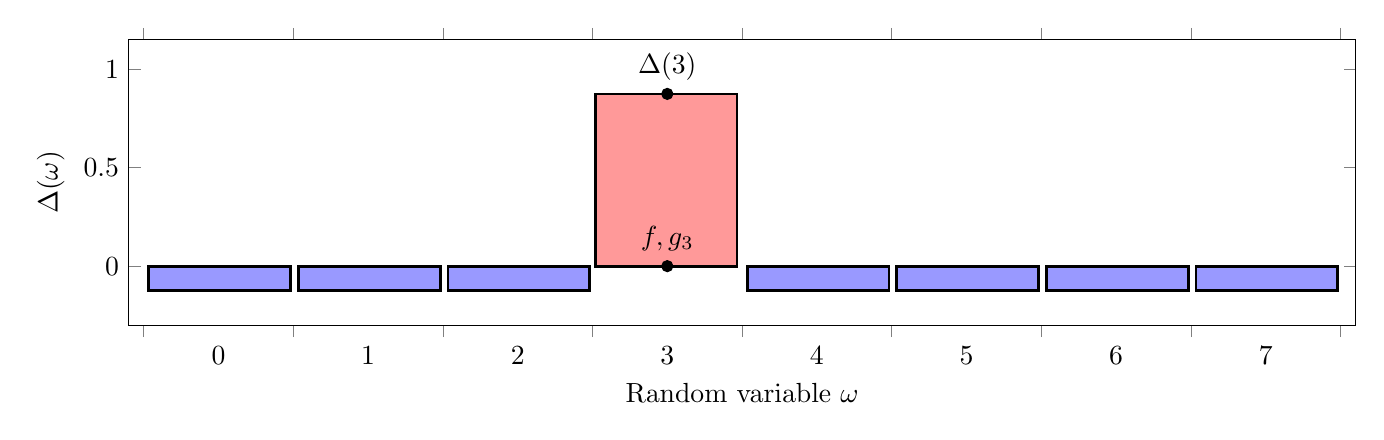
\begin{tikzpicture}
\begin{axis}[
    ybar,
    y=2.5cm,
    x=1.9cm,
    bar width=1.8cm,
    x tick label as interval,
	xtick={0,1,2,3,4,5,6,7,8},
    xmajorgrids=false,    
    xlabel = {Random variable $\omega$},
    ylabel = {$\Delta(\omega)$},
    ymin=-0.3, ymax=1.15,
    xmin=-0.1, xmax=8.1, 
]
\addplot[draw=black, line width=1pt, fill=blue!40] plot 
	coordinates {(1,-0.125) (2,-0.125) (3,-0.125) (5,-0.125) (6,-0.125) (7, -0.125) (8, -0.125)};
\addplot[draw=black, line width=1pt, fill=red!40] plot 
	coordinates {(3, 0.874)};
\addplot+ [ only marks, mark=*, mark options = black] 
	coordinates {(3.5, 0)}
	[yshift=10pt, black]
	node[pos=0]{$\advSemXX{f,g_3}{\AD}$}
;	

\addplot+ [ only marks, mark=*, mark options = black] 
	coordinates {(3.5, 0.875)}
	[yshift=10pt, black]
	node[pos=0]{$\Delta(3)$}
;	
            
\end{axis}
\end{tikzpicture} 
\end{center}
\caption{Counter example that shows that the inequality \eqref{eq:bound} cannot be satisfied by coin-fixing argument}
\label{fig:counter-example}
\end{figure}

\noindent
The presented counter example does not show that it is impossible to choose $\omega\in\Omega$ such that 
\begin{align*}
\advSemXX{f,g}{\AD}\leq \max_{\omega\in\Omega} \set{\advSemXX{f,g_\omega}{\AD}}
\end{align*}
it just shows that there is no easy way to find such coins. To show impossibility of other more clever choice of $\omega$ consider the counter example depicted on Figure~\ref{fig:complete-counter-example}. In this example, the three secrets $\SSS=\set{0,1,2}$ and four equiprobable random values $\Omega=\set{0,1,2,3}$. The function $f$ is deterministic and the adversary $\AD$ is deterministic with the outputs depicted on the figure.  Note that guesses of $\AD$ must coincide on the same row.    

\begin{figure}[!h]
\begin{center}
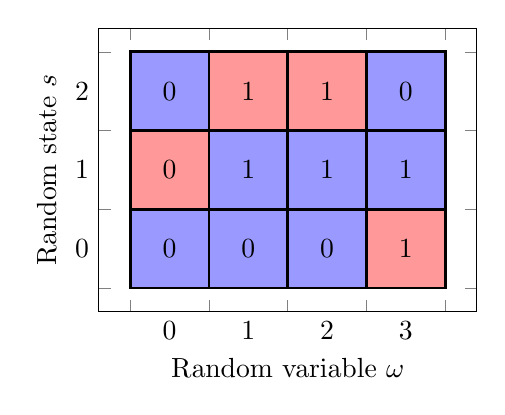
\begin{tikzpicture}
\begin{axis}[
    x=1.0cm,
    y=1.0cm,
    xlabel = {Random variable $\omega$},
    ylabel = {Random state $s$},
    ytick={0,1,2,3},
    y tick label as interval,
    ymajorgrids=false,
    xtick={0,1,2,3,4},
    x tick label as interval,
]
\addplot[draw=black, line width=1pt, fill=blue!40] 
	coordinates {(0,0) (3,0) (3,1) (0,1) (0,0)} 
	\closedcycle;
\addplot[draw=black, line width=1pt, fill=red!40]  
	coordinates {(3,0) (4,0) (4,1) (3,1) (3,0)} 
	\closedcycle;
\addplot[draw=black, line width=1pt, fill=red!40]  
	coordinates {(0,1) (2,1) (2,2) (0,2) (0,1)} 
	\closedcycle;
\addplot[draw=black, line width=1pt, fill=blue!40] 
	coordinates {(1,1) (4,1) (4,2) (1,2) (1,1)} 
	\closedcycle;
\addplot[draw=black, line width=1pt, fill=blue!40] 
	coordinates {(0,2) (0,3) (1,3) (1,2) (0,2)} 
	\closedcycle;
\addplot[draw=black, line width=1pt, fill=red!40] 
	coordinates {(1,2) (1,3) (3,3) (3,2) (1,2)} 
	\closedcycle;
\addplot[draw=black, line width=1pt, fill=blue!40] 
	coordinates {(3,2) (3,3) (4,3) (4,2) (3,2)} 
	\closedcycle;
\addplot[draw=black, line width=1pt]
	coordinates {(1,0) (1,3)}; 
\addplot[draw=black, line width=1pt]
	coordinates {(2,0) (2,3)}; 

\addplot+ [only marks, mark=o, mark size=0pt] 
	coordinates {(0.5, 0.5) (1.5, 0.5) (2.5, 0.5) (3.5, 0.5)}
	[black]
	node[pos=0.00]{$0$}
	node[pos=0.33]{$0$}
	node[pos=0.67]{$0$}
	node[pos=1.00]{$1$};
	
\addplot+ [only marks, mark=o, mark size=0pt] 
	coordinates {(0.5, 1.5) (1.5, 1.5) (2.5, 1.5) (3.5, 1.5)}
	[black]
	node[pos=0.00]{$0$}
	node[pos=0.33]{$1$}
	node[pos=0.67]{$1$}
	node[pos=1.00]{$1$};

\addplot+ [only marks, mark=o, mark size=0pt] 
	coordinates {(0.5, 2.5) (1.5, 2.5) (2.5, 2.5) (3.5, 2.5)}
	[black]
	node[pos=0.00]{$0$}
	node[pos=0.33]{$1$}
	node[pos=0.67]{$1$}
	node[pos=1.00]{$0$};
\end{axis}
\end{tikzpicture} 
\end{center}
\caption{Counter example that shows that the inequality \eqref{eq:bound} cannot be satisfied at all. All squares are equiprobable in the experiment. The number inside the square marks the output of $g(s,\omega)$. Correct guesses are marked with blue  and incorrect guesses are marked with red squares.}
\label{fig:complete-counter-example}
\end{figure}
\noindent
Since $\AD$ guesses the value $g(s,\omega)$ on eight squares and there are equal number of ones and zeros, we get
\begin{align*}
\advSemXX{f,g}{\AD}={\textstyle\frac{8}{12}-\frac{1}{2}=\frac{1}{6} }\enspace.
\end{align*}
As $\AD$ guesses correctly only two values in each row, $\pr{\smash{\GAME_{0\omega_*}^\AD=1}}=\frac{2}{3}$.  
If the randomness is fixed then the best choice for $y_\circ$ can be determined by majority voting and thus $ \pr{\smash{\GAME_{1\omega_*}^\AD=1}} \geq\frac{2}{3}$. The latter implies that
$\advSemXX{f,g_\omega}{\AD}\leq 0$ for any $\omega\in\set{0,1,2,3}$ and thus $\advSemXX{f,g}{\AD}>\advSemXX{f,g_\omega}{\AD}$. 
\end{solution}
\end{document}